
\section{Timing Measurements} 
\label{sec:timing} 

We characterize the timing performance of the CdTe sensor by measuring the timestamps
relative to the MCP-PMT device used as a reference timer. An example of the distribution 
of the timestamp measurement for $100$~GeV electrons after $6$~$\mathrm{X}_{0}$ of absorber
material is shown in Figure~\ref{fig:DeltaT}. We extract the time measurement
resolution from this distribution as the width parameter of a Gaussian fit.
In Figure~\ref{fig:TimeResolutionVsEnergy} we show the measured time resolution as a function of the
beam energy. For beam energies below $50$~GeV, the time resolution improves
with increasing signal size as expected based on the increasing signal-to-noise ratio.
However, above $100$~GeV, the time resolution no longer improves with 
increasing signal size, which points towards some systematic limitation. 
We study a number of such factors in Section~\ref{sec:systematicLimitations} below.

%Fig: example DeltaT plot
\begin{figure}[htbp] 
\centering
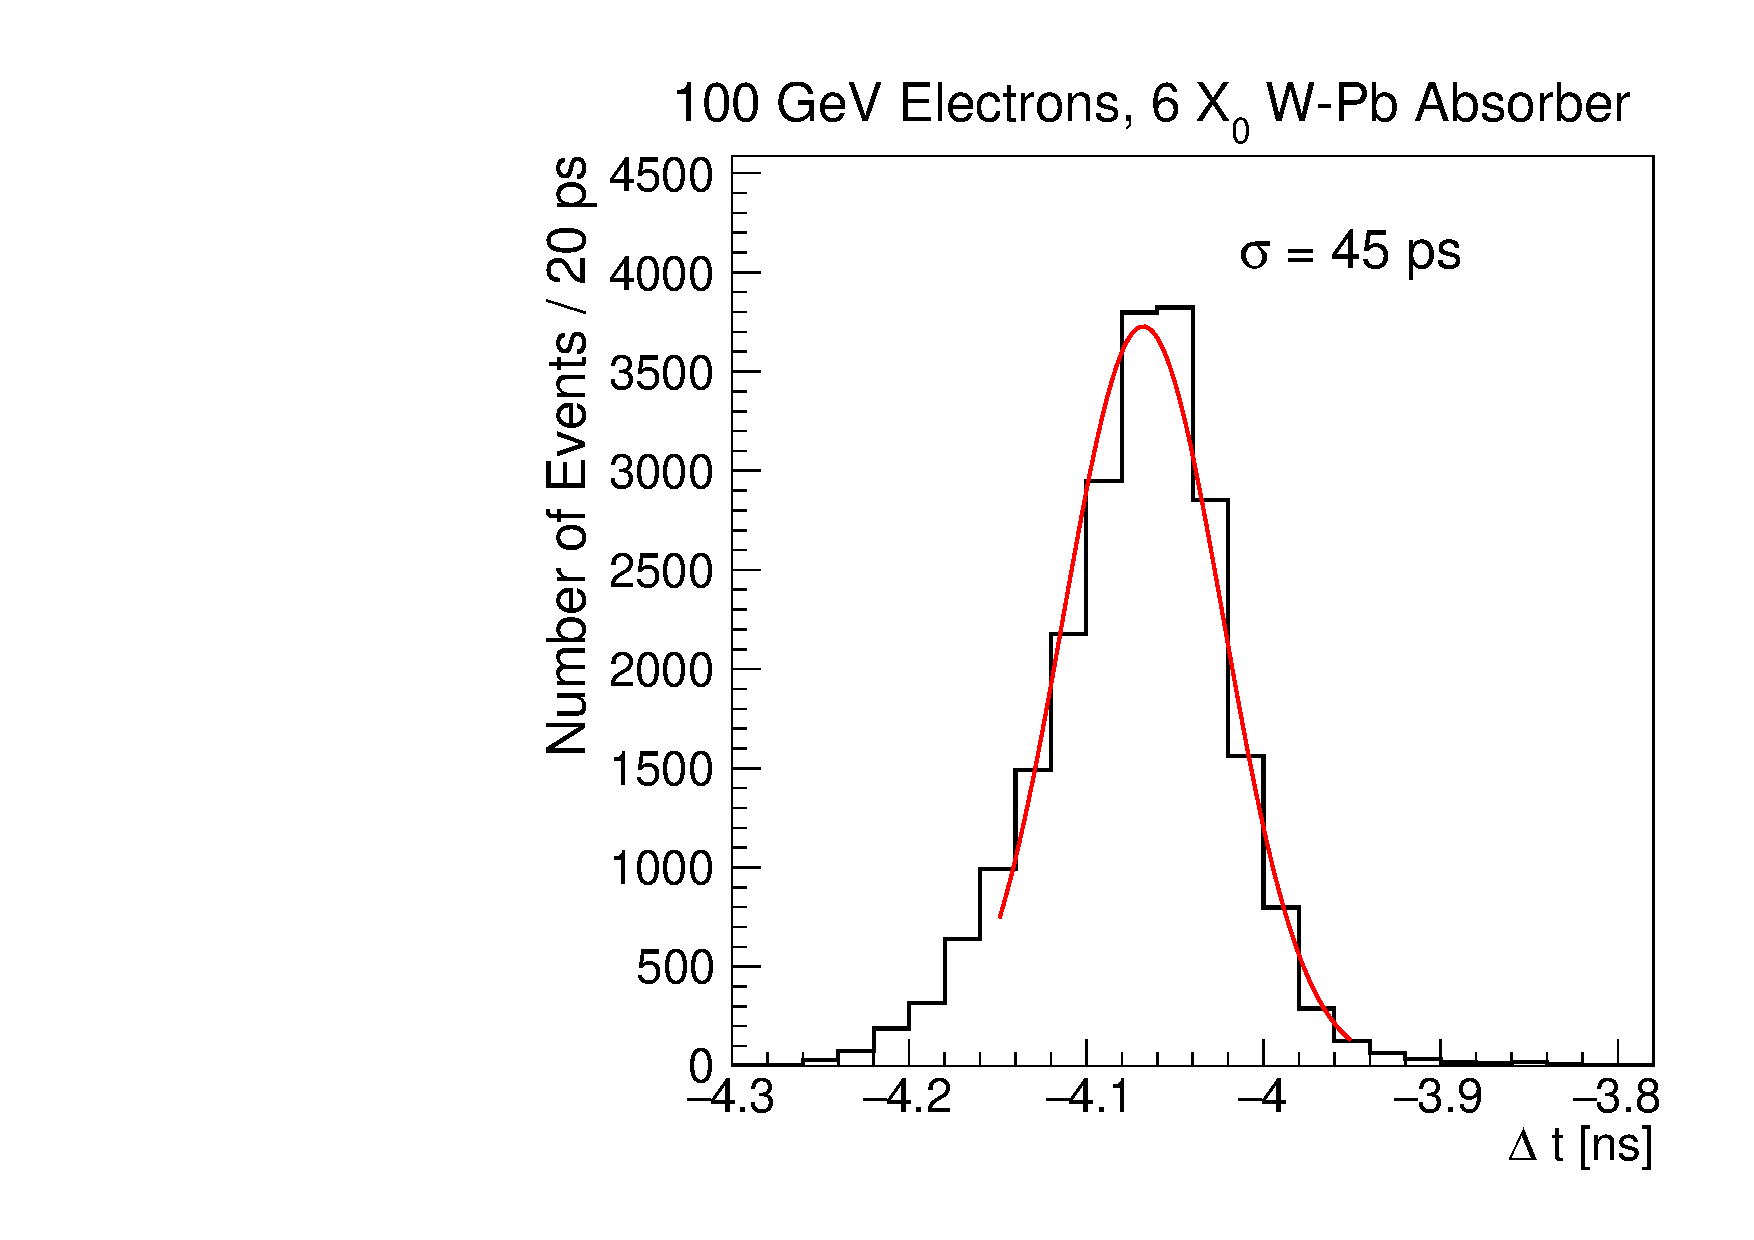
\includegraphics[width=0.49\textwidth]{figures/100GeV_deltaT.pdf} 
\caption{Distribution of the timestamp measurement in the CdTe sensor for a $100$~GeV
electron after $6$~$\mathrm{X}_{0}$ of tungsten and lead absorber. } 
\label{fig:DeltaT} 
\end{figure} 


%Fig: Time resolution vs beam energy
\begin{figure}[htbp] 
\centering
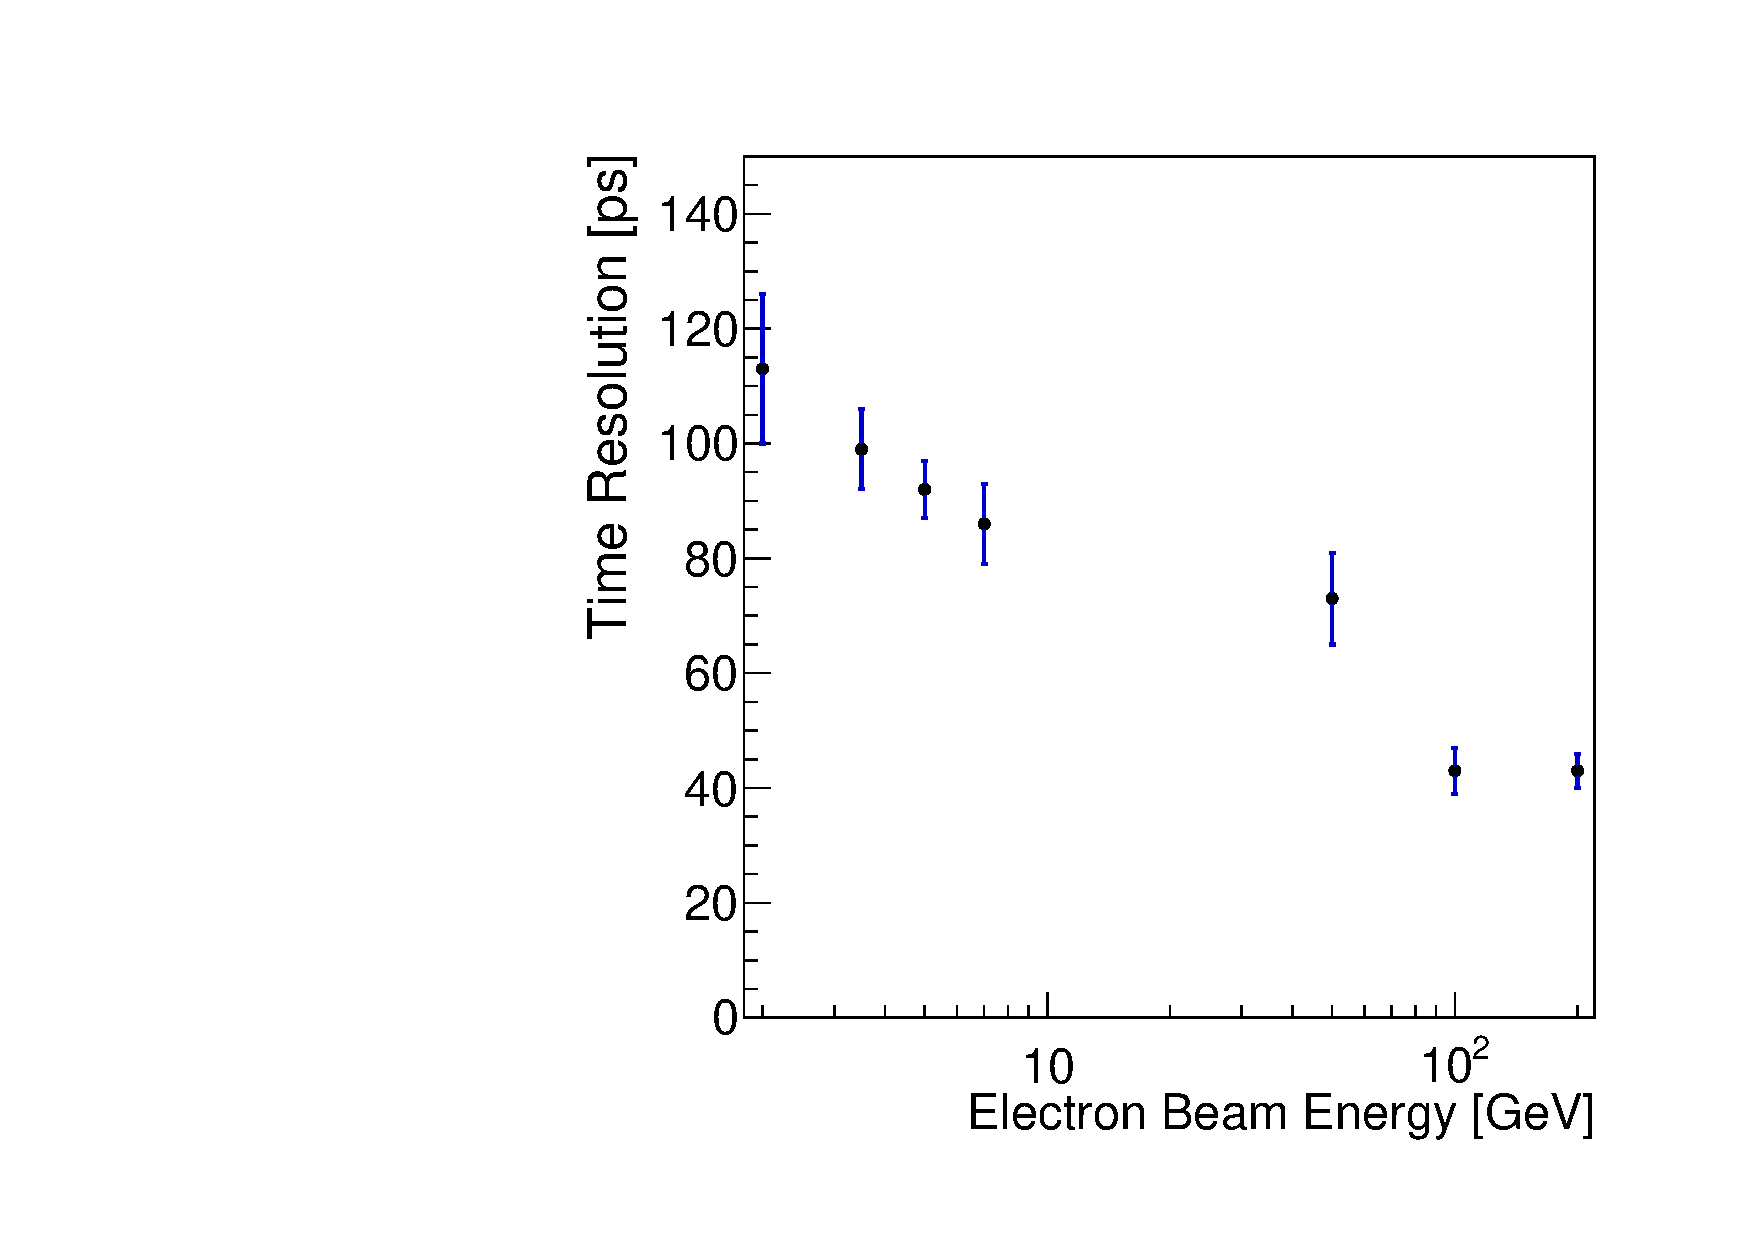
\includegraphics[width=0.49\textwidth]{figures/TimeResolutionVsEnergy.pdf} 
\caption{ The measured time resolution of the CdTe sensor is plotted as a function
of the electron beam energy. } 
\label{fig:TimeResolutionVsEnergy} 
\end{figure} 


To further characterize the timing performance of the CdTe signals, we measure the
risetime, defined as the time for the signal to rise from $10\%$ to $90\%$ of its maximum
amplitude, for various electron beam energies. The distribution of risetime for
$100$~GeV electrons and the measured risetime as a function of the beam energy
are shown on the left and right of Figure~\ref{fig:riseTime} respectively. 
We observe a risetime of around $1.3$~ns that does not vary significantly
with the beam energy.


%Fig: riseTime vs energy
\begin{figure}[htbp] 
\centering
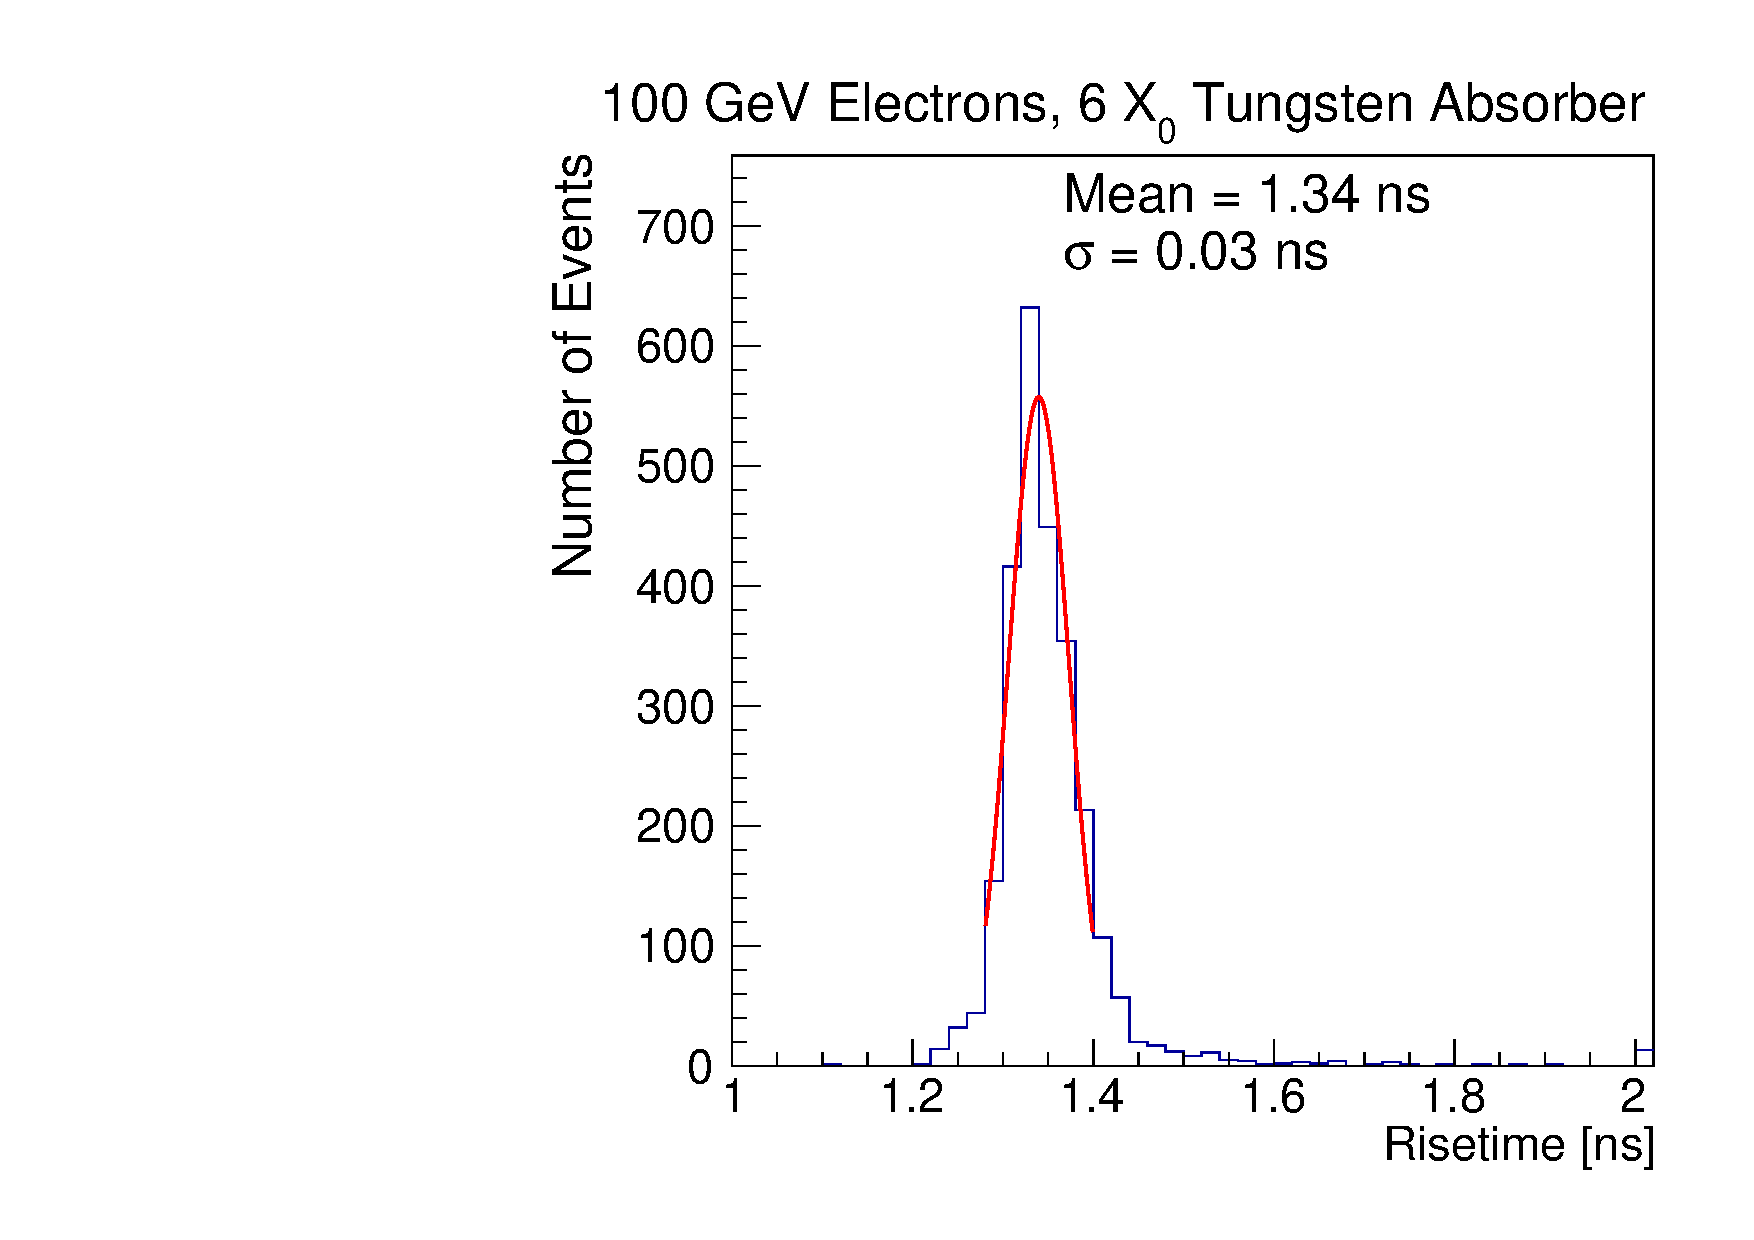
\includegraphics[width=0.488\textwidth]{figures/100GeV_risetime.pdf} 
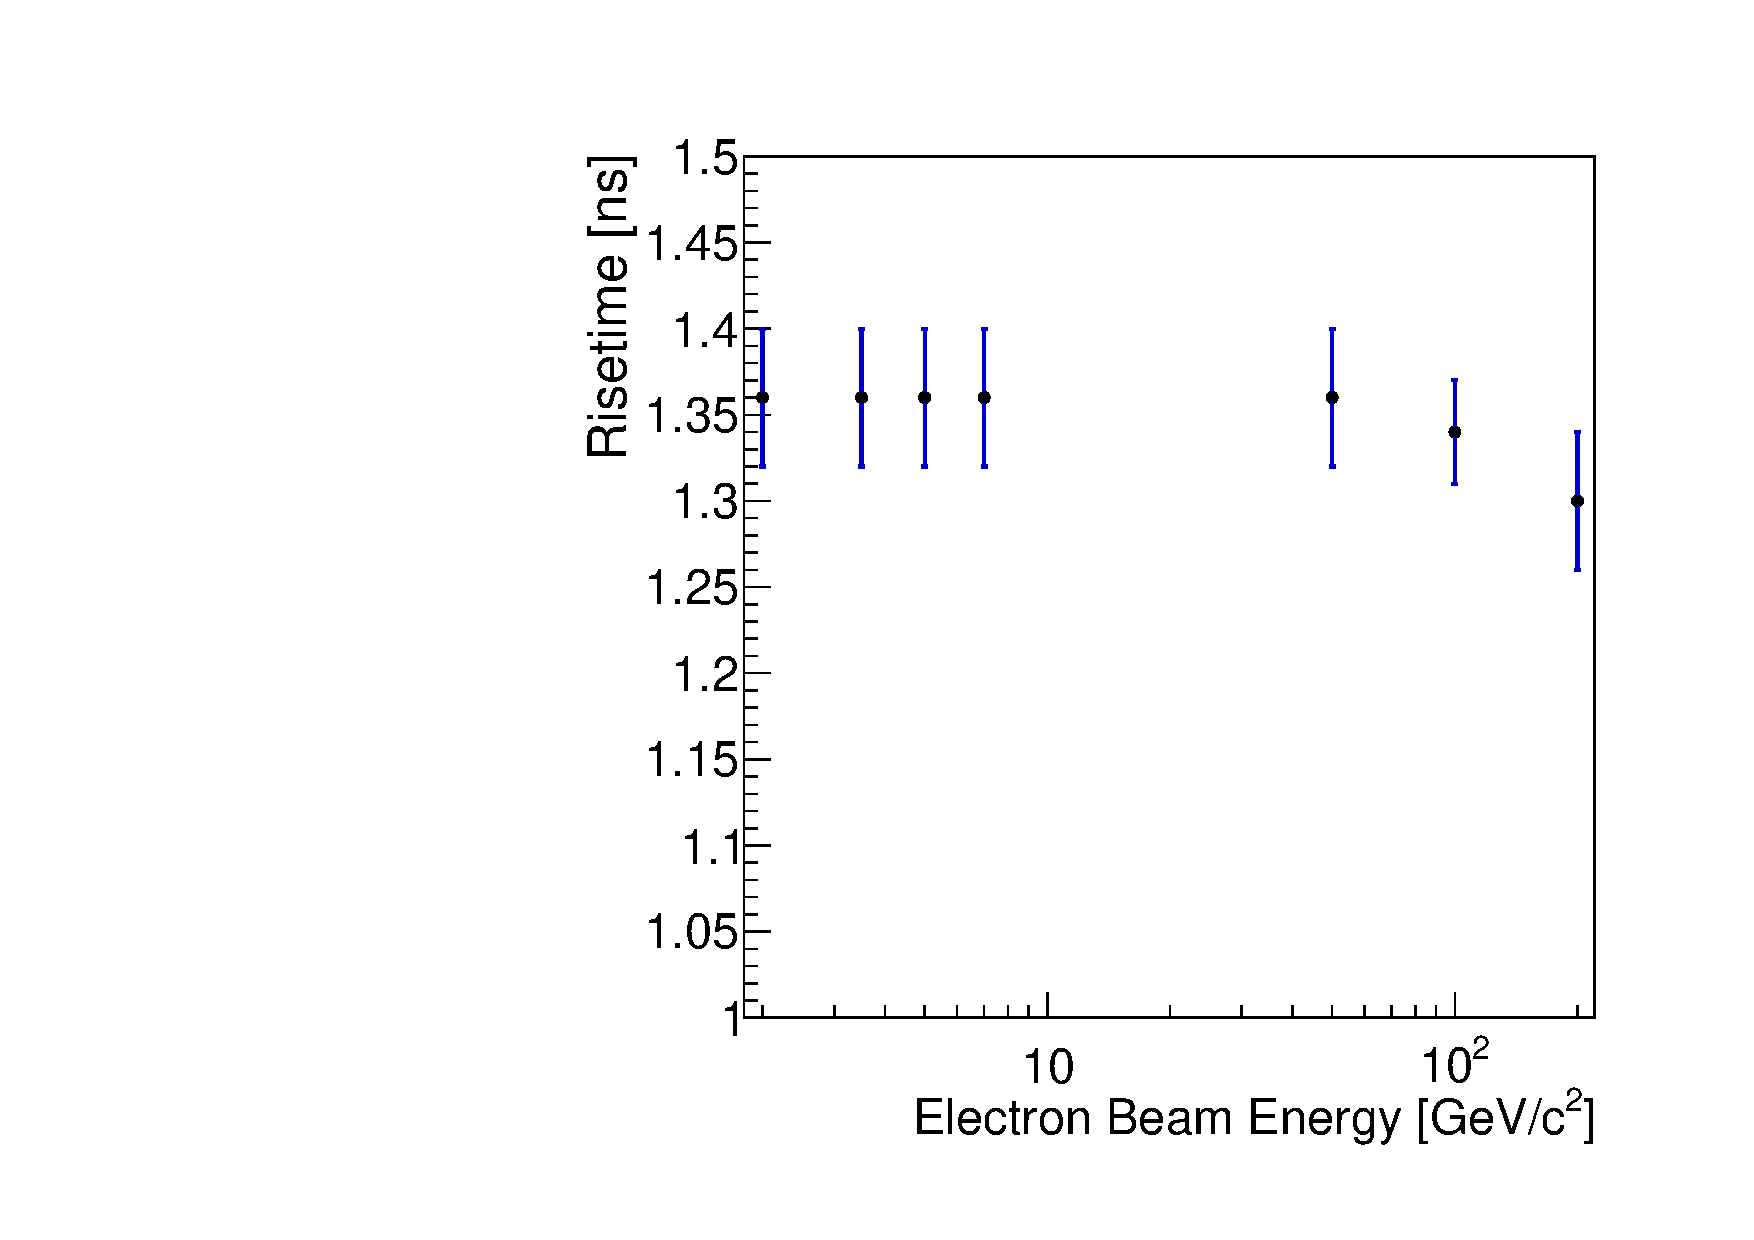
\includegraphics[width=0.518\textwidth]{figures/RisetimeVsEnergy.pdf} 
\caption{ Left: Distribution of risetime of the CdTe signal for $100$~GeV electrons. 
Right: Risetime of the CdTe signal is plotted as a function of the incident beam energy. } 
\label{fig:riseTime} 
\end{figure} 



\subsection{Studies of Systematic Limitations on Time Resolution}
\label{sec:systematicLimitations}

One of the major systematic effects that have been observed in past
timing studies~\cite{Anderson:2015gha,Ronzhin201552,MCPShowerMaxPaper} is the dependence 
of the time measurement on the amplitude of the signal. On the left of 
Figure~\ref{fig:DeltaTVsAmplitude}, we show the dependence of the timestamp measurement 
on the amplitude of the signal, and observe a mild dependance on amplitude, which we correct for
in subsequent figures.
On the right of Figure~\ref{fig:DeltaTVsAmplitude}, we show the measured time resolution
as a function of the signal amplitude and we observe a clear improvement
in the resolution with increasing signal amplitudes up to $0.5$~V.
In this region, the impact of the signal-to-noise ratio is still 
the dominant factor for the time resolution.

%Fig: DeltaT vs Amplitude
\begin{figure}[htbp] 
\centering
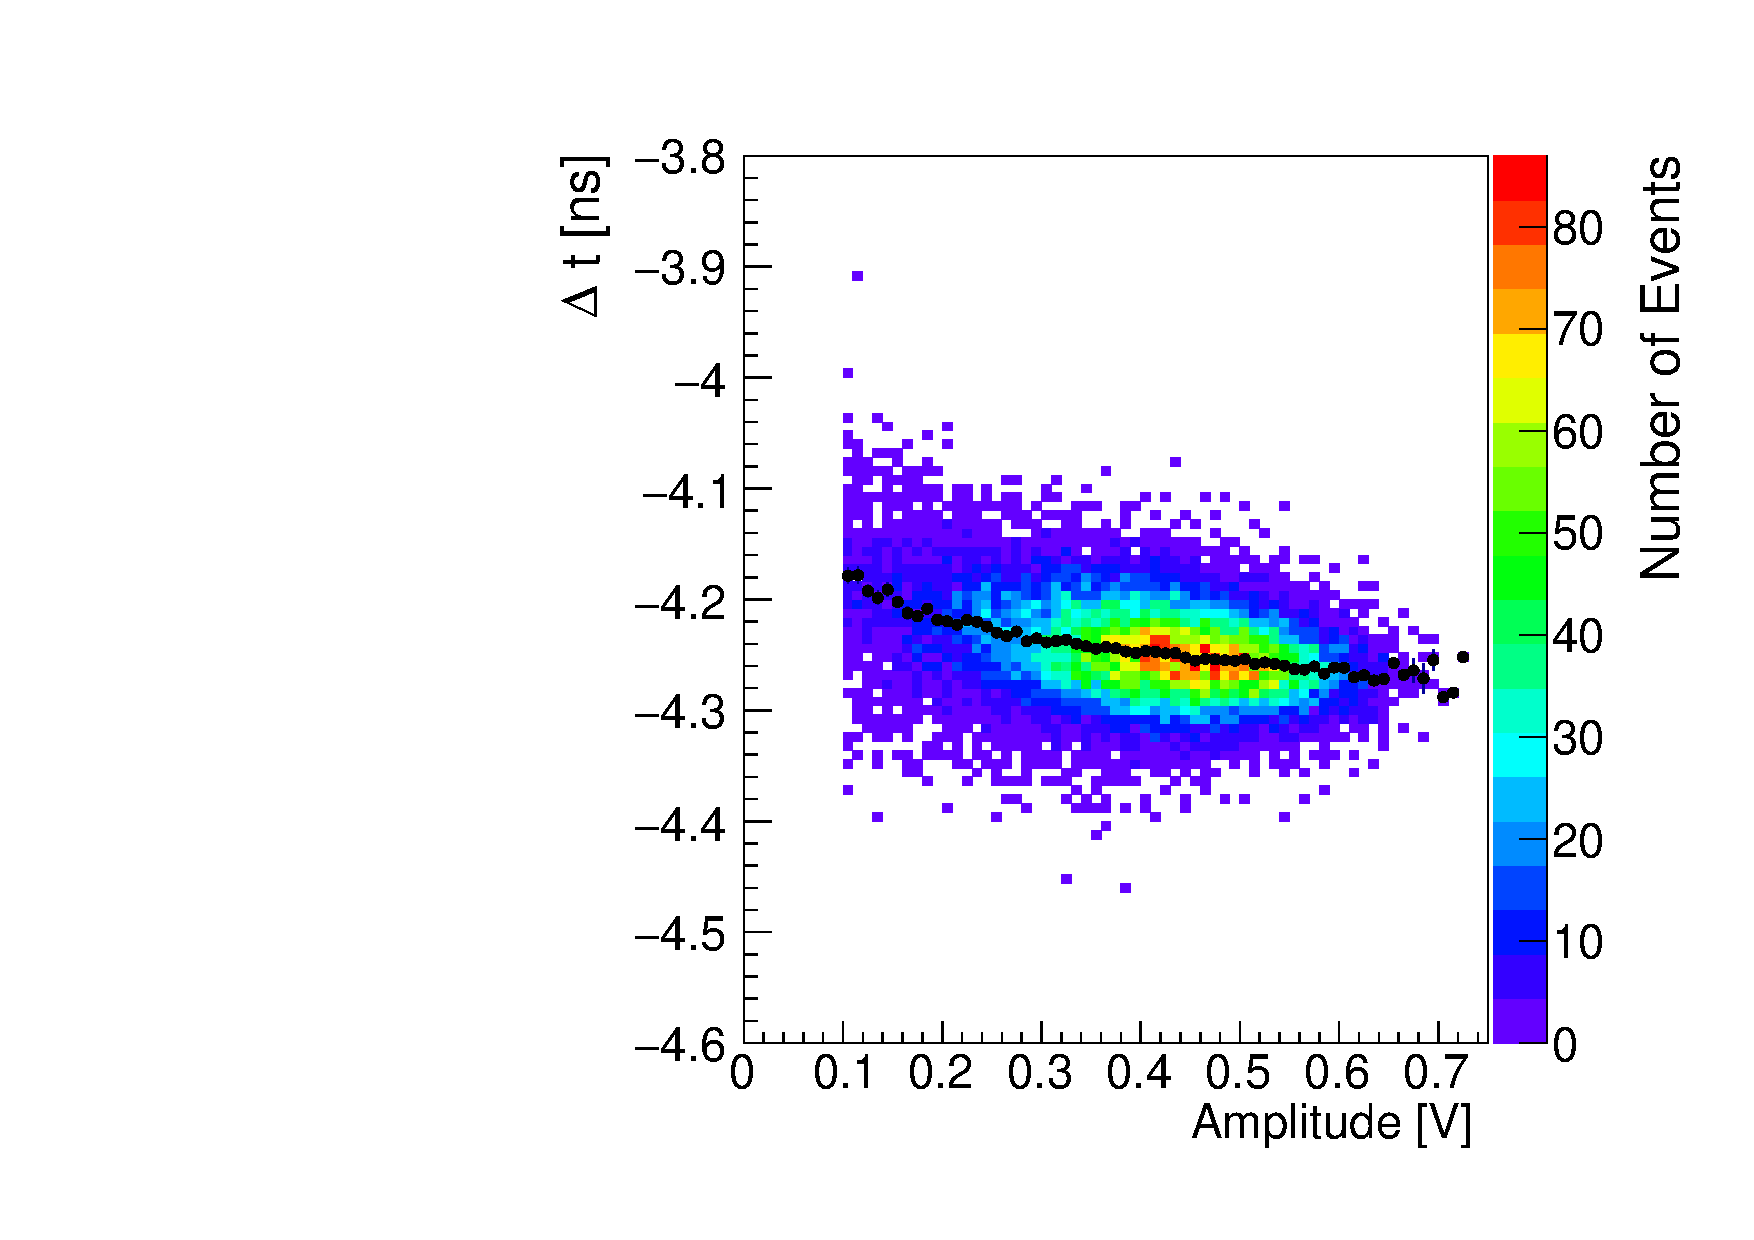
\includegraphics[width=0.49\textwidth]{figures/100GeV_deltaTVsAmp.pdf} 
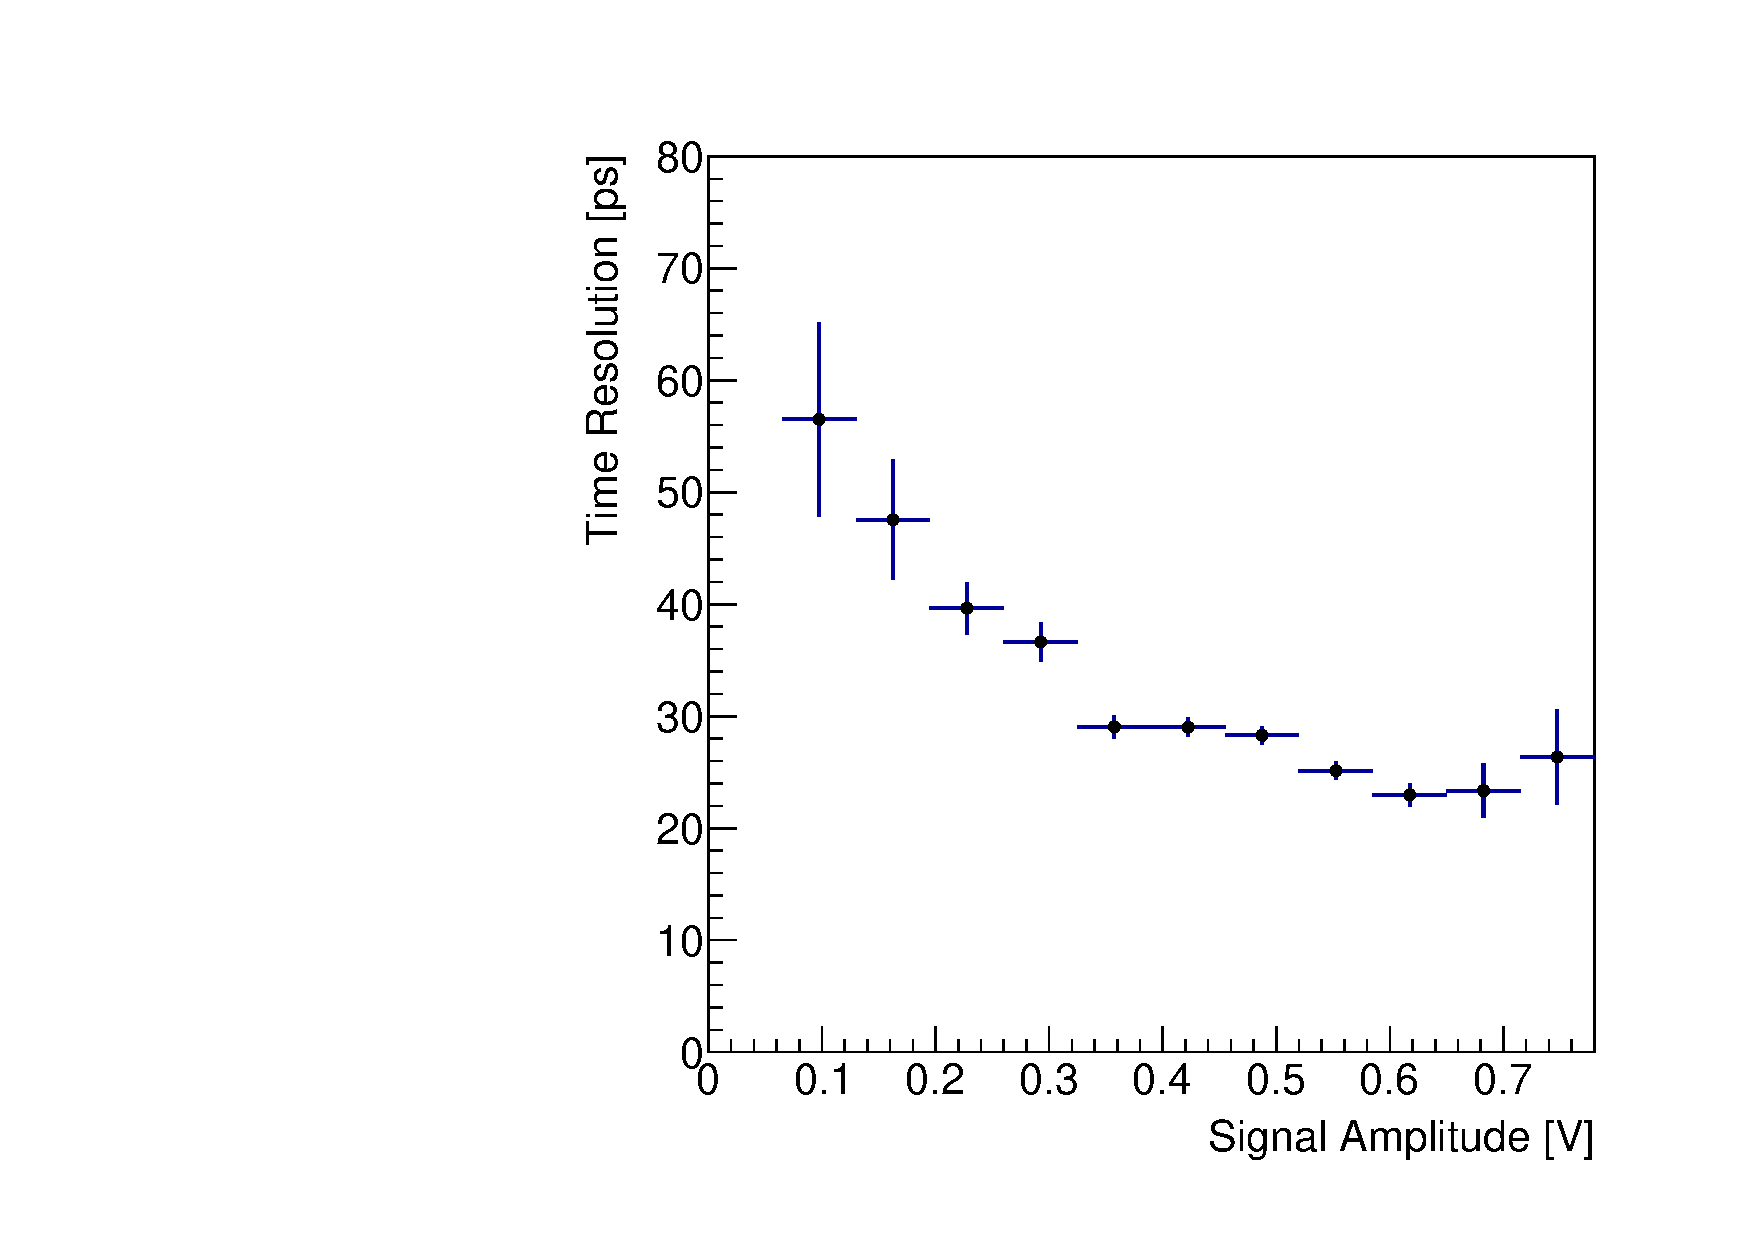
\includegraphics[width=0.49\textwidth]{figures/TimeResolutionVsAmplitude.pdf} 
\caption{ Left: The distribution of the signal amplitude in the CdTe sensor and 
the time measured in the CdTe sensor relative to the Photek reference detector
is shown in the color scale. This data is from a $100$~GeV electron beam after $6$~$X_0$ absorber.
The mean value of the time measured in the CdTe sensor 
as a function of the signal amplitude is shown in the black points. 
Right: The time resolution is measured as a function of the signal amplitude after correction
for amplitude non-linearity. } 
\label{fig:DeltaTVsAmplitude} 
\end{figure} 


We also study the dependence of the timestamp measurement as a function of the geometric
position of the incident beam particle as measured by the wire chambers in 
Figure~\ref{fig:DeltaTVsBeamXY}. A relatively large and linear dependence is observed, 
and this position non-uniformity of the time response adds significantly to the 
time resolution (about $37$~ps). Performing a correction for this non-uniformity improves
the time resolution from $45$~ps to $25$~ps for events with $100$~GeV electrons.
The distribution of timestamps after correcting for the geometric position is shown
in Figure~\ref{fig:DeltaTCorr}. The measured time resolution, after correction for
the position non-uniformity, has a mild dependence on the beam particle position 
and is shown in Figure~\ref{fig:TimeResolutionVsBeamXY}. Combining the time resolution
dependence on the horizontal and vertical beam positions, we measure the time resolution
as a function of the planar distance between the beam position and the location of the 
back wire bond on the CdTe sensor, and observe a more clear dependence shown in 
Figure~\ref{fig:TimeResolutionVsR}. More detailed studies are necessary
to derive a better understanding of this effect. It will be crucial for any precision timing device
using planar semi-conductor sensors to study the uniformity of the response to achieve an optimal performance.
%
%Fig: DeltaT vs Beam Location
\begin{figure}[htbp] 
\centering
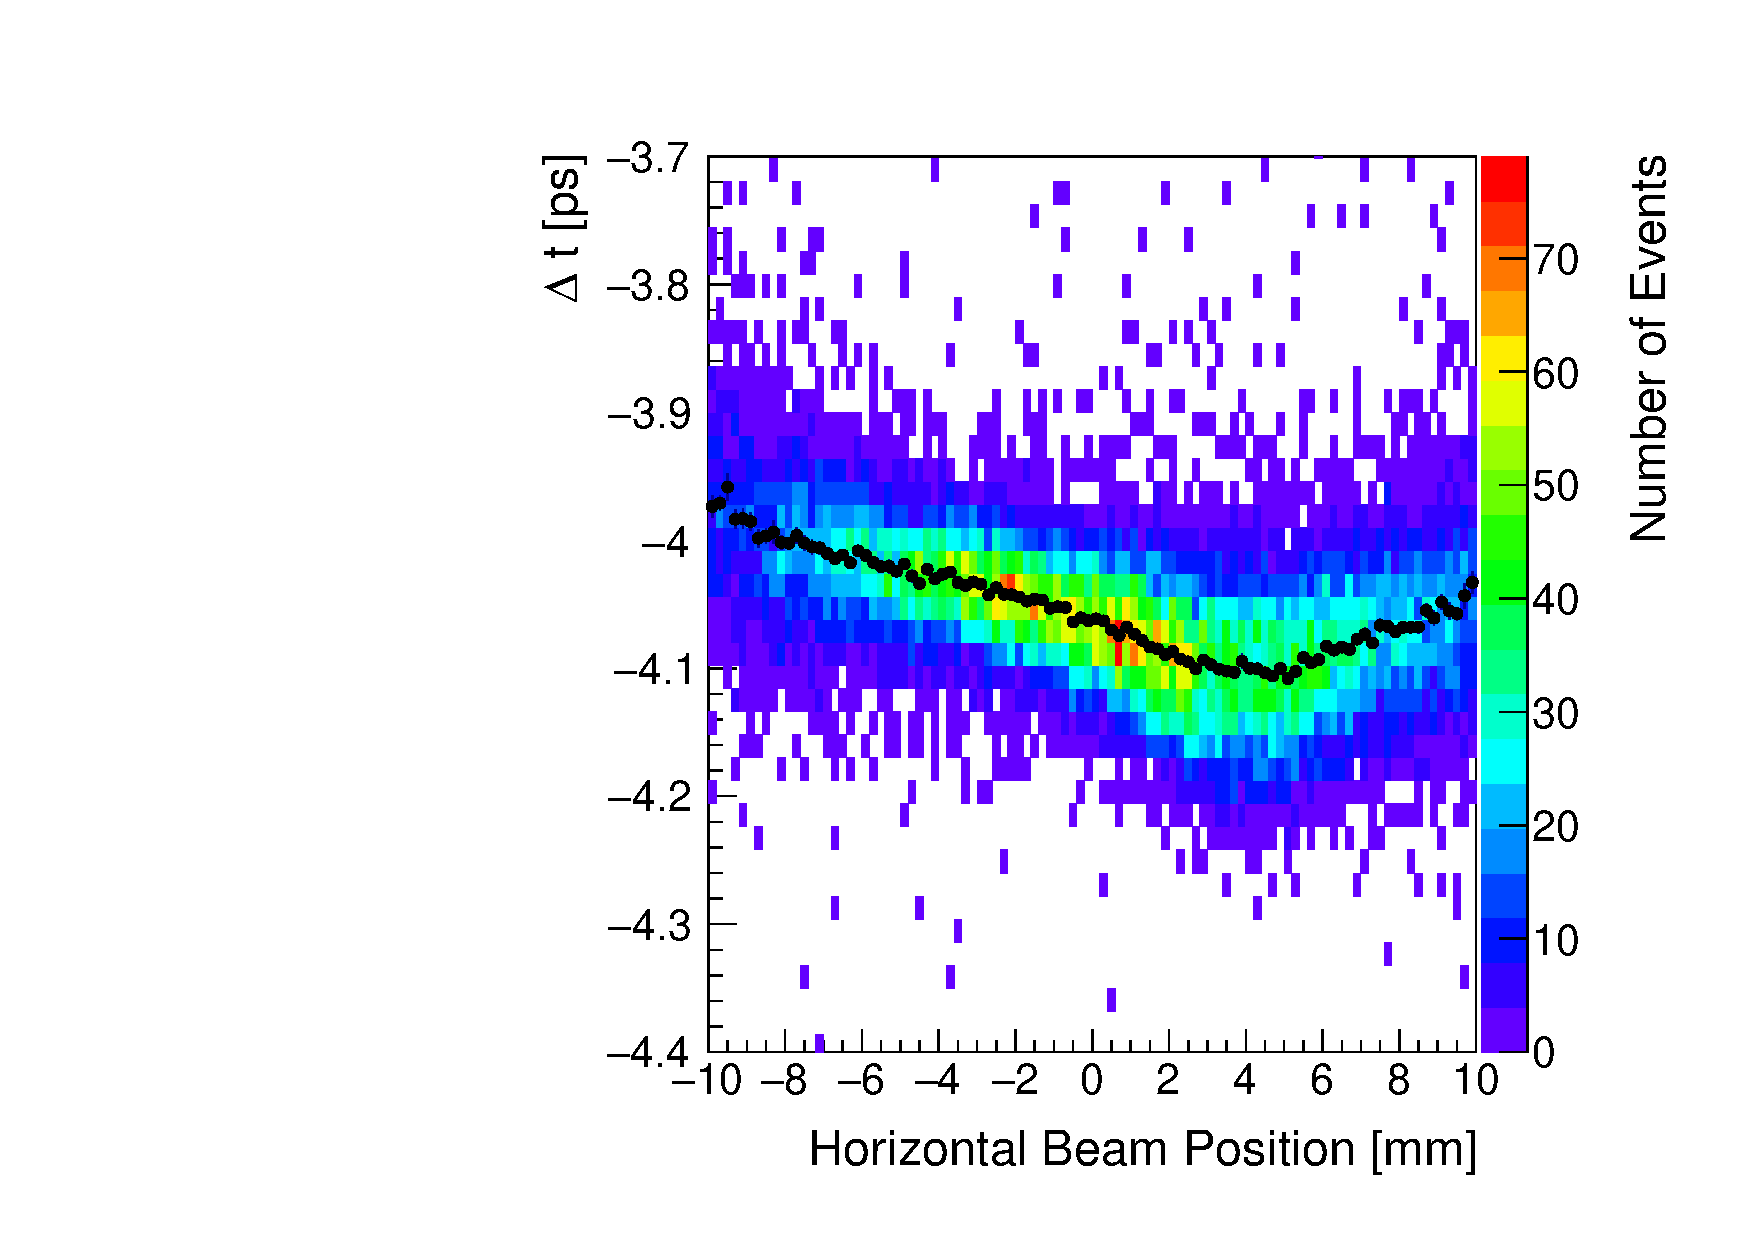
\includegraphics[width=0.49\textwidth]{figures/DeltaTVsHorizontalPosition.pdf} 
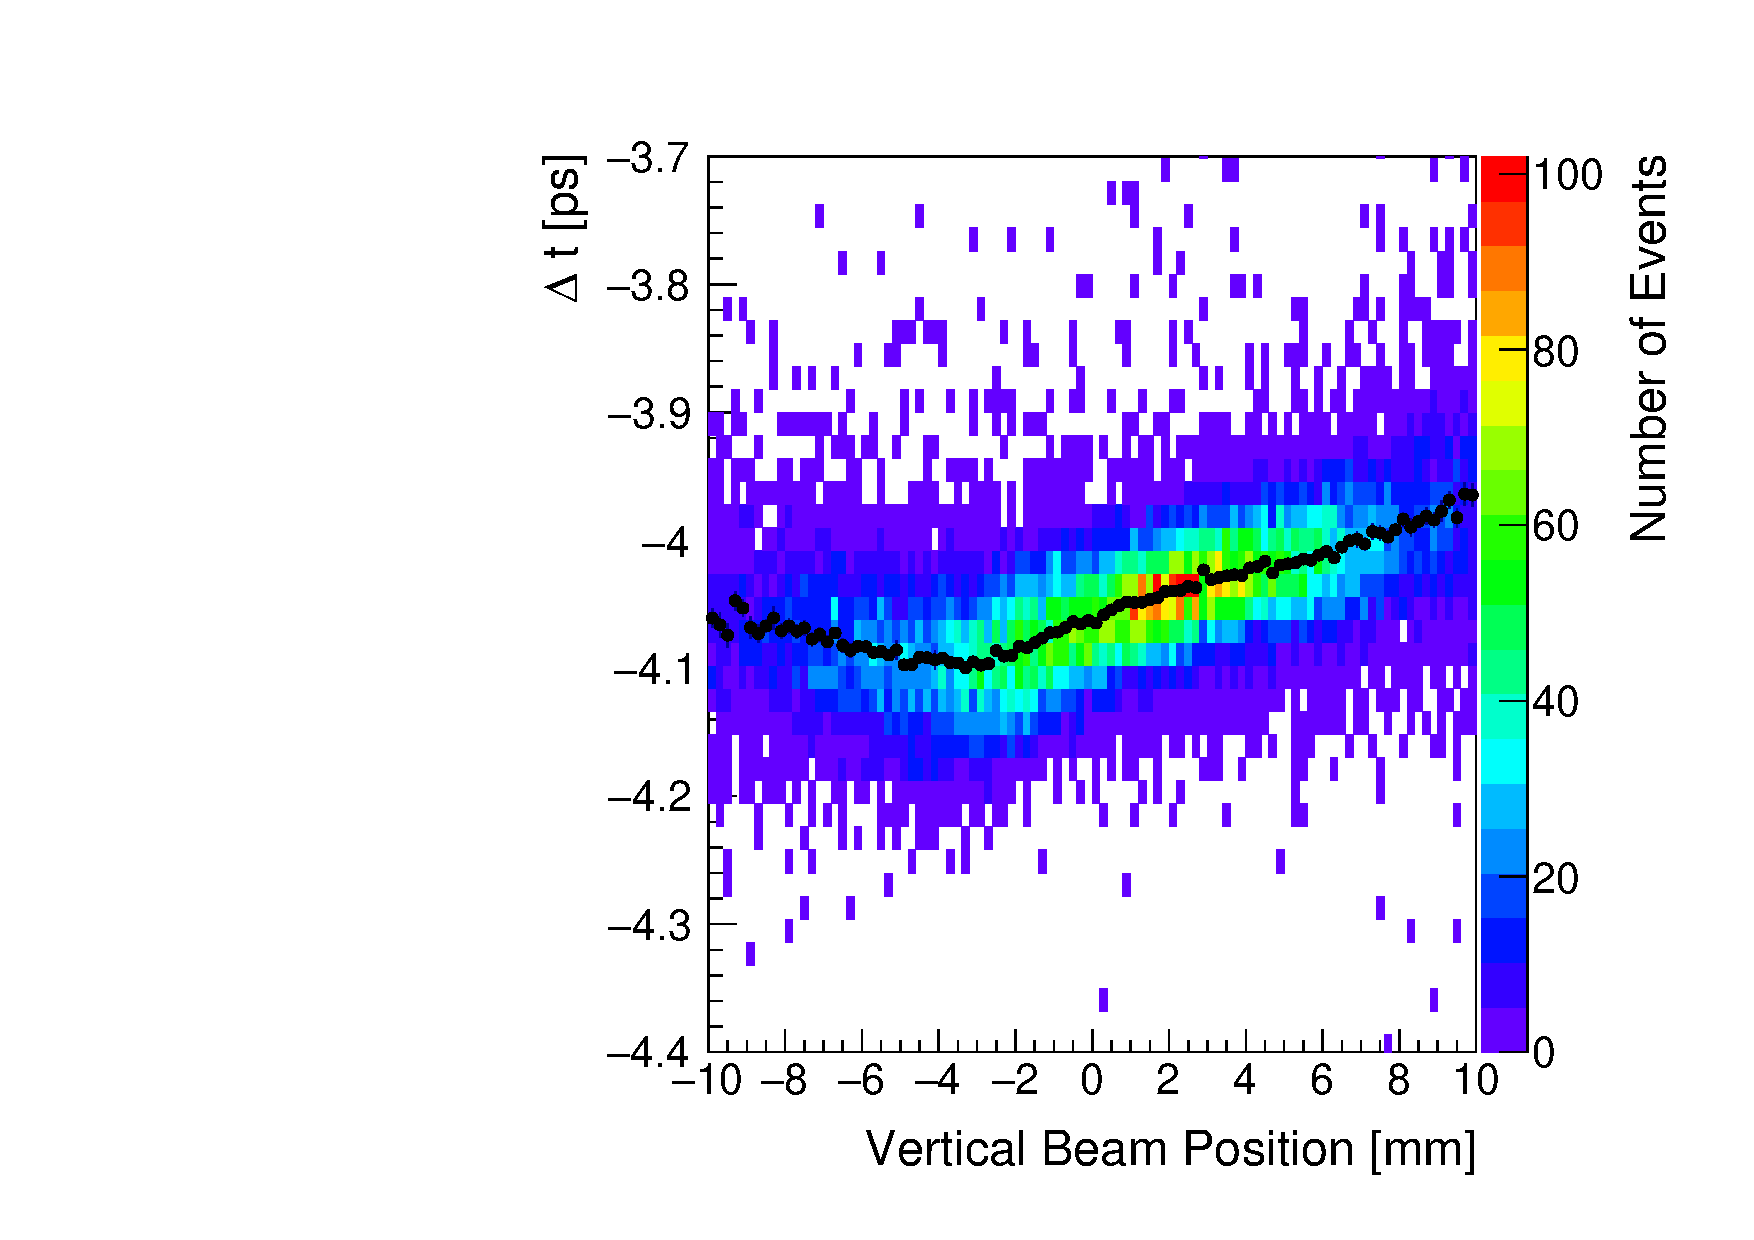
\includegraphics[width=0.49\textwidth]{figures/DeltaTVsVerticalPosition.pdf} 
\caption{ The distribution of the beam particle position measured by the wire chamber
and the time measured in the CdTe sensor relative to the Photek reference detector
is shown in the color scale. The mean value of the time measured in the CdTe sensor as a function
of the beam particle position is shown in the black points. There is a dependence of the time difference
on the impact point on the CdTe sensor which corresponds to about 100 ps across the CdTe sensor.} 
\label{fig:DeltaTVsBeamXY} 
\end{figure} 

\begin{figure}[htbp] 
\centering
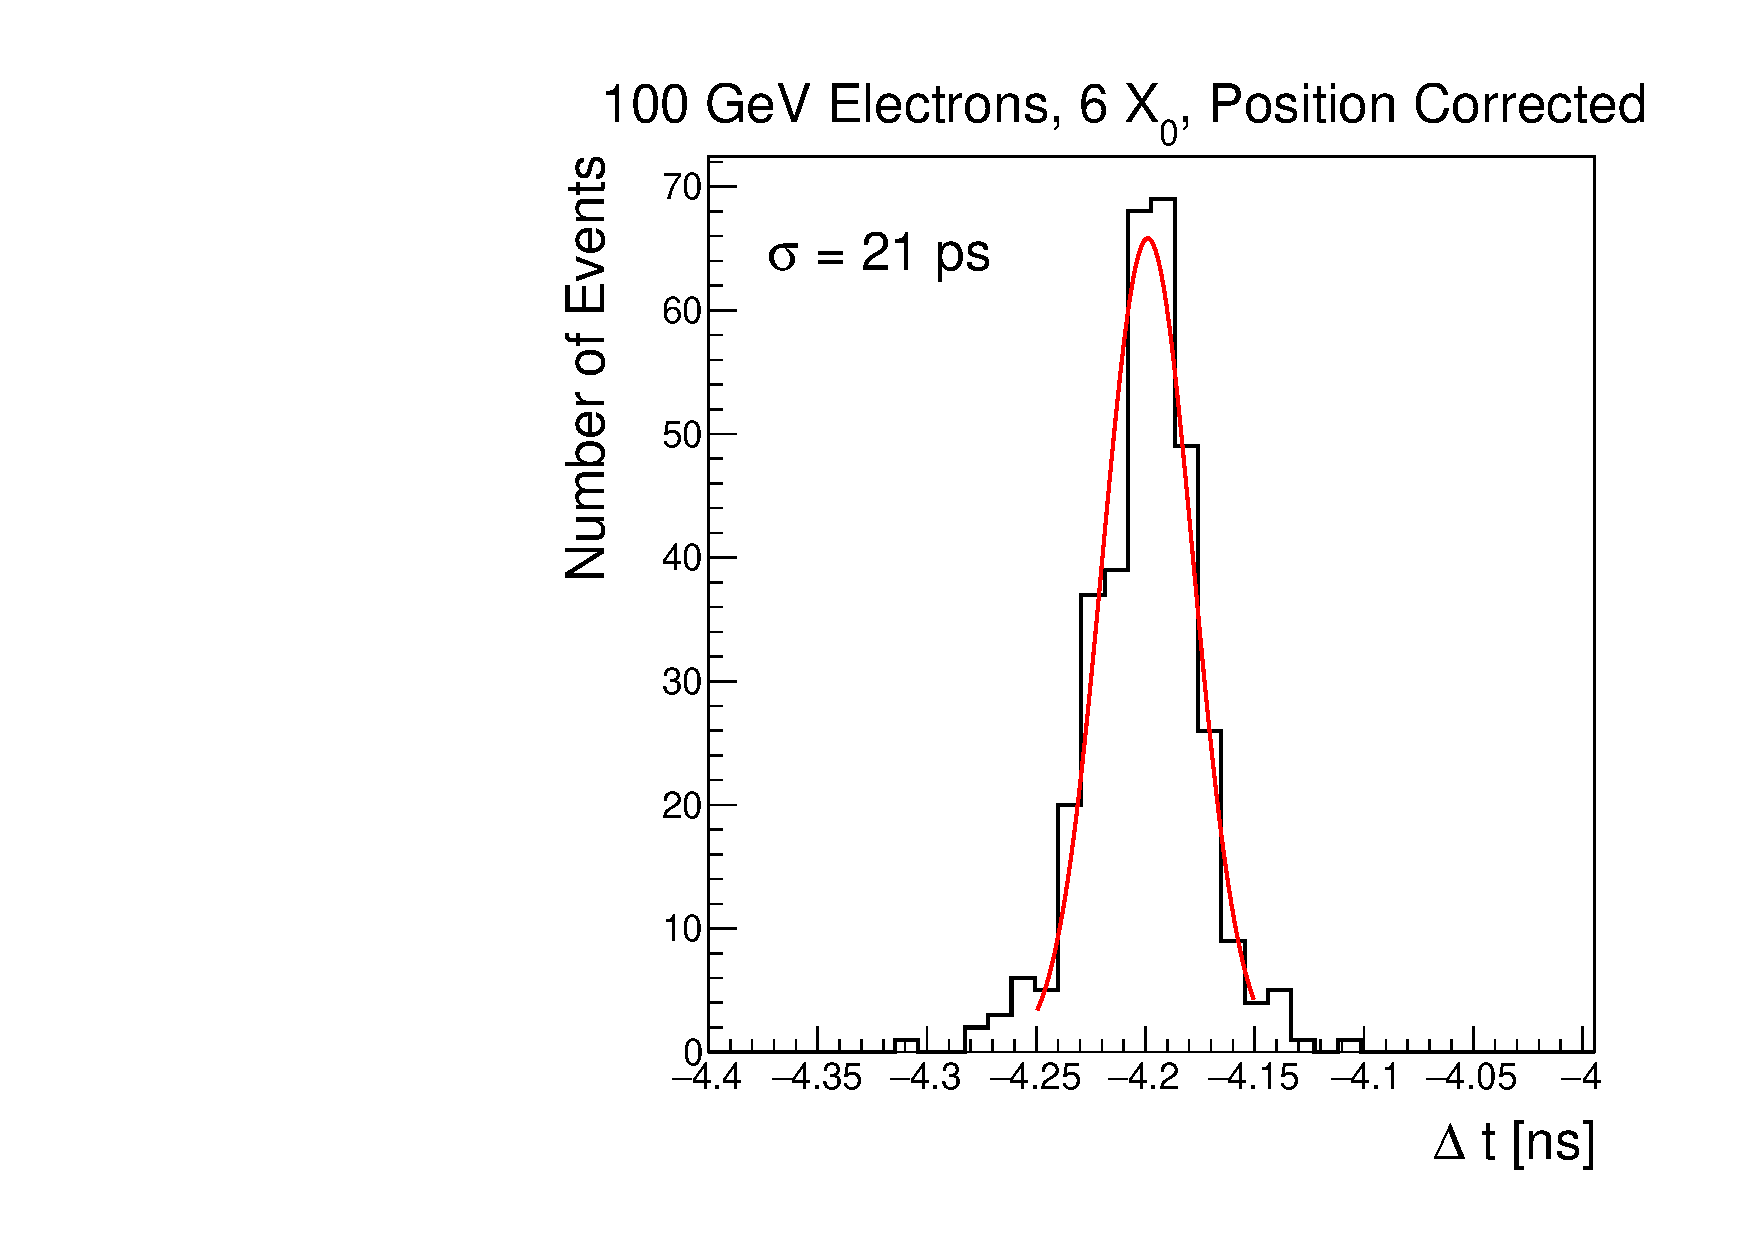
\includegraphics[width=0.49\textwidth]{figures/CdTeTimingResolution_100GeV_PositionCorrected.pdf} 
\caption{Distribution of the timestamp measurement corrected for the geometric position
non-uniformity in the CdTe sensor for a $100$~GeV electron after $6$~$\mathrm{X}_{0}$ of tungsten absorber. } 
\label{fig:DeltaTCorr} 
\end{figure} 



%Fig: Time Resolution vs Beam Location
\begin{figure}[htbp] 
\centering
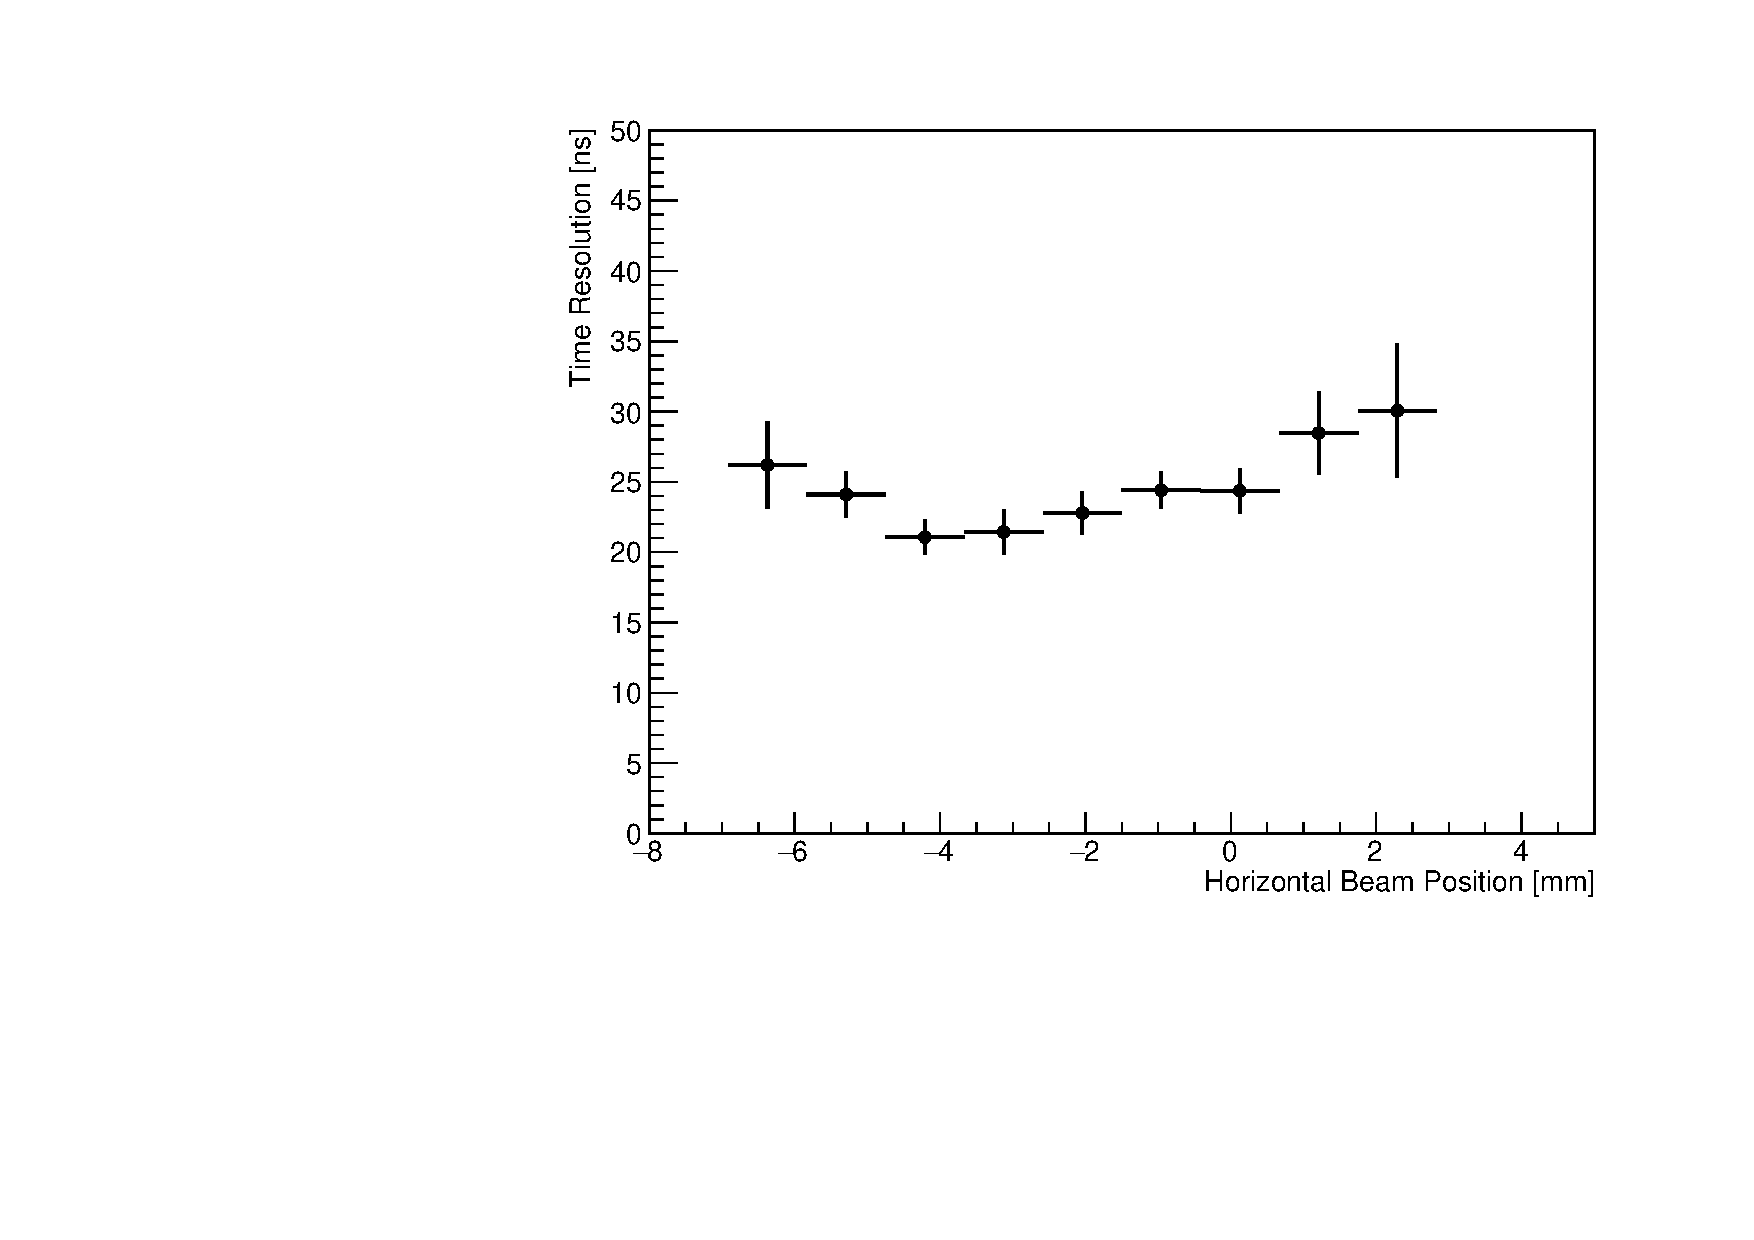
\includegraphics[width=0.49\textwidth]{figures/TimeResolutionVsBeamHorizontalPosition.pdf} 
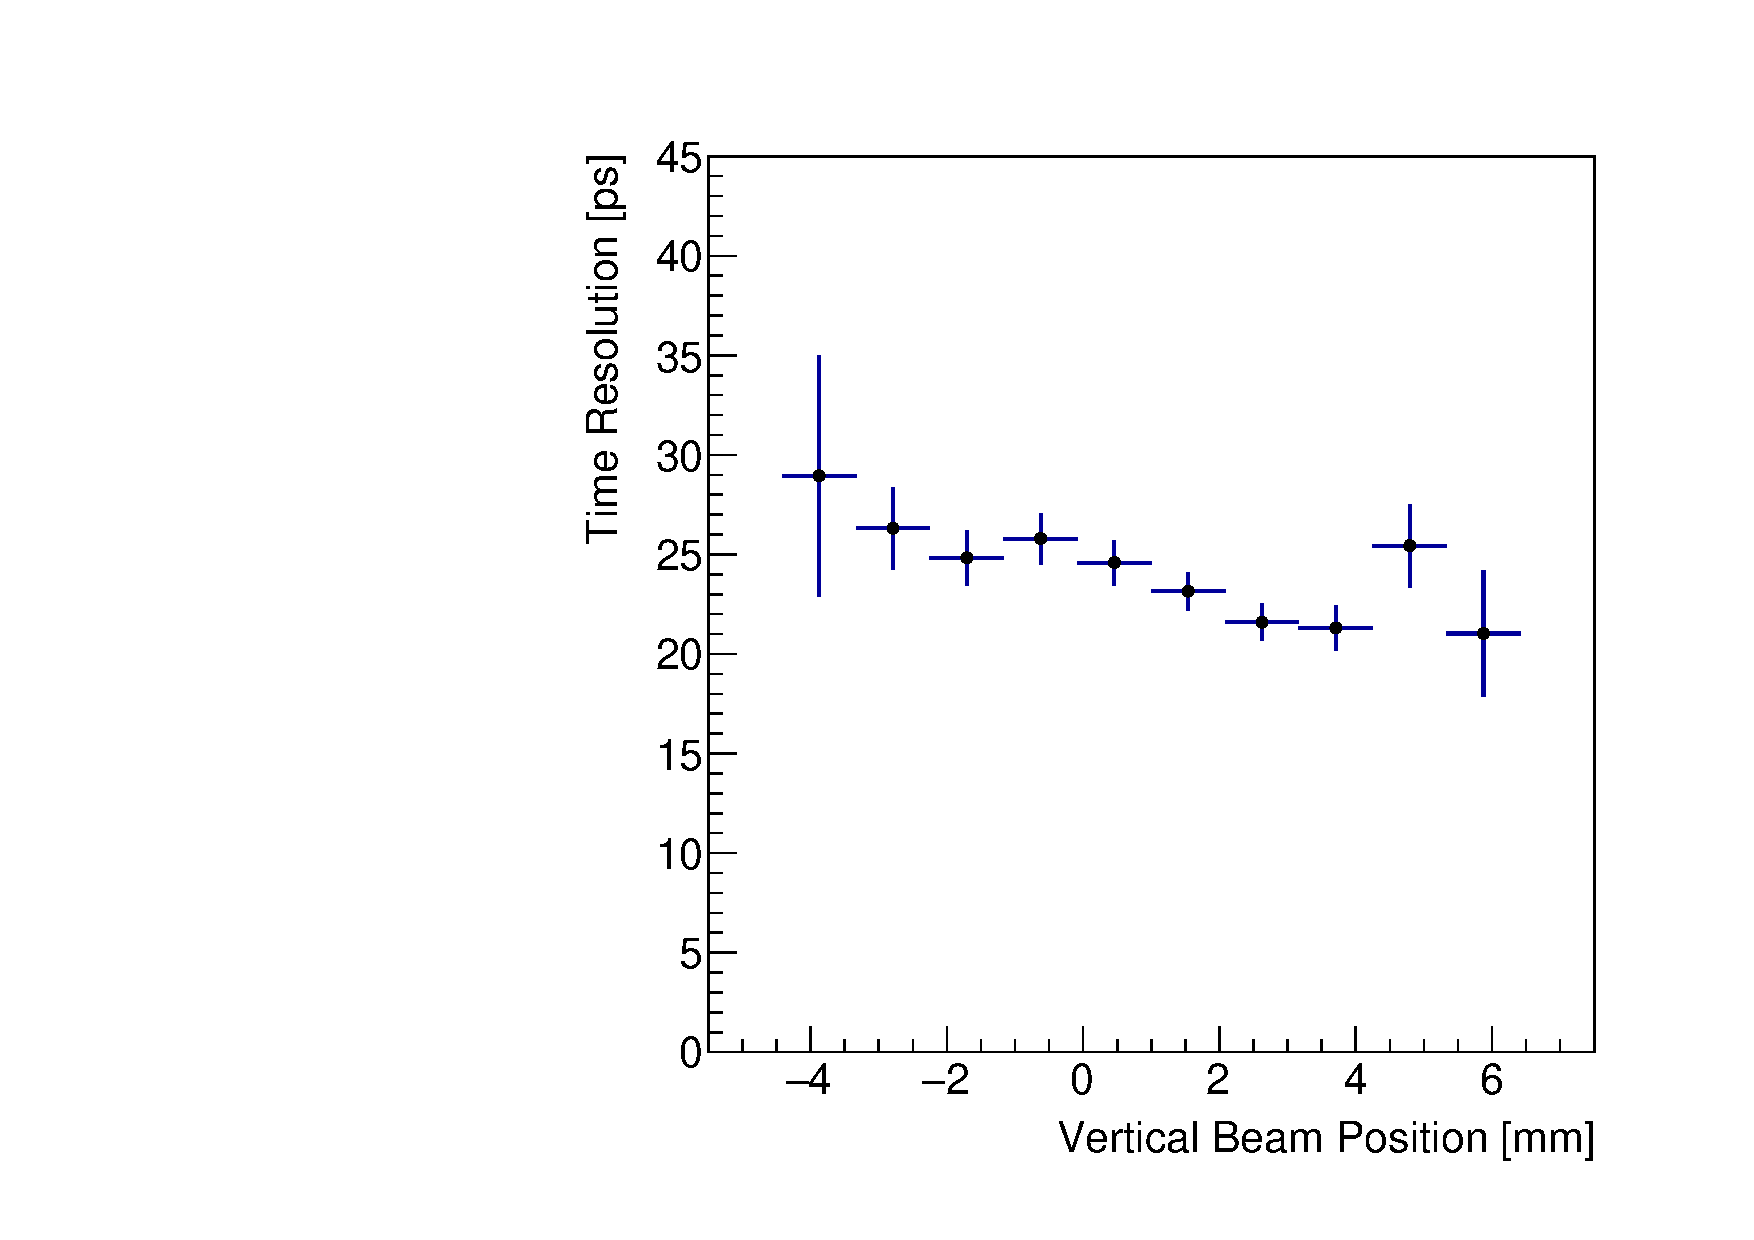
\includegraphics[width=0.49\textwidth]{figures/TimeResolutionVsBeamVerticalPosition.pdf} 
\caption{ The time resolution is measured as a function of the horizontal (left) and vertical (right)
beam position in a 2 mm wide fiducial region around the center of the sensor in the vertical (left) 
and horizontal (right) directions respectively. }
\label{fig:TimeResolutionVsBeamXY} 
\end{figure} 


%Fig: Time Resolution vs Anode Wire Bond Location  
\begin{figure}[htbp]
\centering 
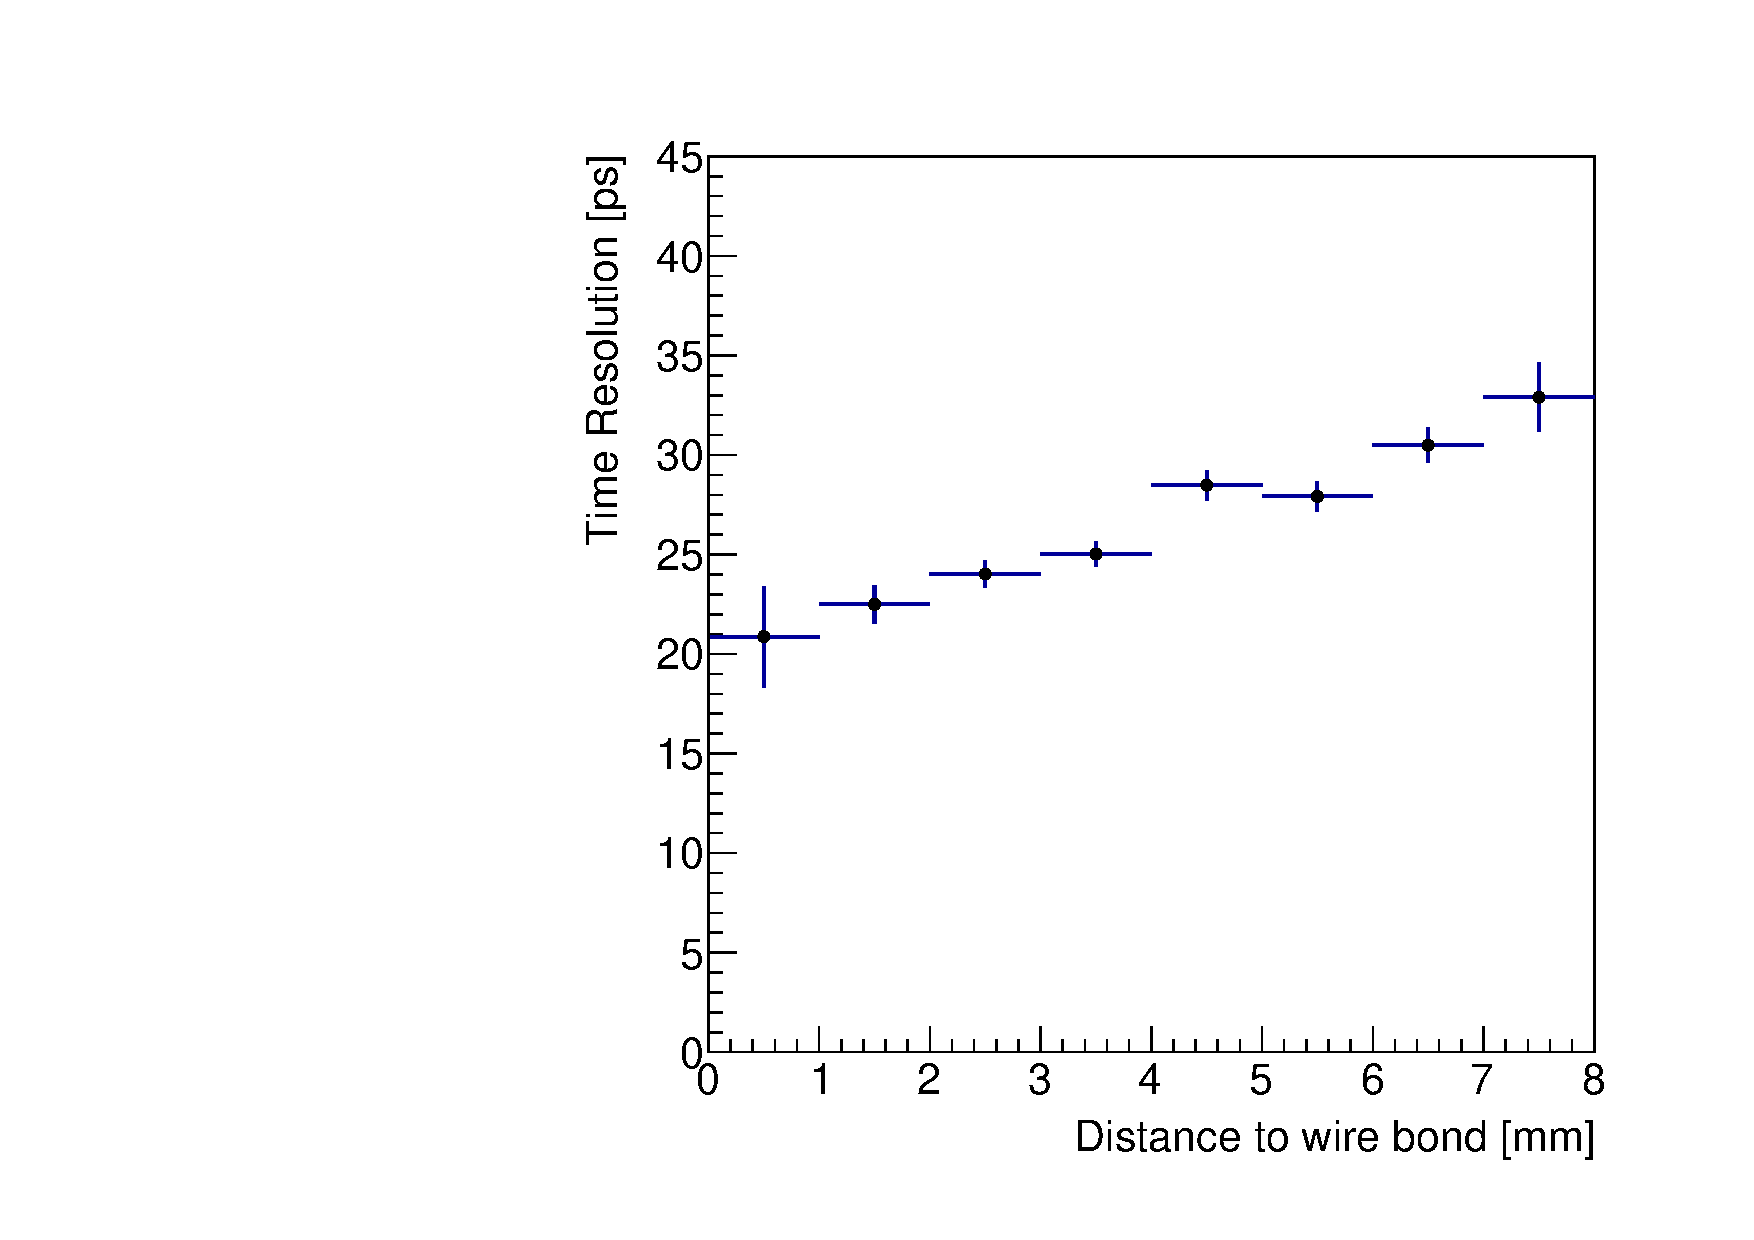
\includegraphics[width=0.49\textwidth]{figures/TimeResolutionVsR.pdf} 
\caption{ The time resolution is measured as a function of the planar distance of the 
incident beam particle to the back wire bond location on the sensor. The position non-uniformity
of the time response as shown in Fig.~\ref{fig:DeltaTVsBeamXY} has been corrected for. There 
remains a dependence of the measured resolution across the sensor, reaching 20 ps in the location
closest to the back wire bond connection.}
\label{fig:TimeResolutionVsR}
\end{figure}




%Extra studies
%MIP peak
%Charge vs beam location ( can we say anything about signal size on shower periphery? )
